\documentclass[conference]{IEEEtran}
\IEEEoverridecommandlockouts

\usepackage{cite}
\usepackage{amsmath,amssymb,amsfonts}
\usepackage{graphicx}
\usepackage{booktabs}
\usepackage{multirow}
\usepackage{textcomp}
\usepackage{xcolor}
\usepackage{url}

% Highlight unfinished parts so they are easy to find
\newcommand{\todo}[1]{\textcolor{red}{[TODO: #1]}}

\graphicspath{{figures/}{../results/figures/}}

\begin{document}

\title{Product Review Rating Prediction:\\
Comparing Ordinal Loss Functions for TextCNN and DistilBERT\\
\large CS415 Progress Report}

\author{\IEEEauthorblockN{Efe Han Kele\c{s}}
\IEEEauthorblockA{\textit{Computer Science and Engineering} \\
\textit{Sabanc{\i} University} \\
efe.keles@sabanciuniv.edu}
\and
\IEEEauthorblockN{Ege A\c{s}an}
\IEEEauthorblockA{\textit{Computer Science and Engineering} \\
\textit{Sabanc{\i} University} \\
ege.asan@sabanciuniv.edu}
\and
\IEEEauthorblockN{Faris Aleem Ahmad}
\IEEEauthorblockA{\textit{Computer Science and Engineering} \\
\textit{Sabanc{\i} University} \\
faris.ahmad1@sabanciuniv.edu}
}

\maketitle

\begin{abstract}
Predicting a 1--5 star rating from review text is an ordinal problem, but the usual cross-entropy loss treats a one-star and a four-star error alike. We compare cross entropy with two ordinal losses, Ordinal Log Loss (OLL) and Multitask Log Loss (MLL), on two architectures, a TextCNN with fixed GloVe vectors and a fine-tuned DistilBERT, using the Amazon Fine Food Reviews data split by product. This progress report covers the data pipeline, the implementation, and one run of each of the six settings. With TextCNN, OLL lowers the MAE by 5.4\% and the share of errors of two or more stars by 17.4\%, without losing Macro F1. A class-weighted linear baseline gives gains of similar size, so part of this benefit may come from correcting the bias towards 5 stars. With DistilBERT, which is stronger overall, the ordinal losses give no clear gain (OLL: MAE +2.8\%, large errors $-6.7\%$, Macro F1 $-0.018$). These results come from a single seed; three seeds, tuning of the loss parameters and a larger DistilBERT training budget remain to be done.
\end{abstract}

\begin{IEEEkeywords}
rating prediction, ordinal classification, TextCNN, DistilBERT, ordinal log loss
\end{IEEEkeywords}

\section{Problem Definition and Motivation}
\label{sec:intro}

Online shops collect huge numbers of product reviews. The text tells us about a customer's experience, and the star rating sums up how satisfied they were. In this project we predict the star rating of a review, from 1 to 5, from its text alone. A model like this could estimate a rating for a written review that has none, and it could also help to check whether a rating and its text actually agree.

\subsection{Why the Task Is Difficult}
A single review often contains both positive and negative opinions, for example praise for the taste of a product together with a complaint about its price. Similar comments can also receive different ratings, because customers have different expectations. In addition, the data is strongly imbalanced: in the dataset we use, about 64\% of the reviews give five stars and only about 5\% give two stars (Section~\ref{sec:experiments}). So a model can get a high accuracy just by favoring the majority class, which means accuracy alone says little about how good it is.

\subsection{Why the Order of the Ratings Matters}
Star ratings are ordered. Predicting 2 stars for a 1-star review is a smaller mistake than predicting 5 stars. Standard training with cross entropy ignores this order: every wrong class is penalized the same way. Ordinal losses such as Ordinal Log Loss (OLL)~\cite{castagnos2022} and Multitask Log Loss (MLL)~\cite{kasa2024} add a penalty that grows with the distance between the predicted and the true rating. The evaluation should reflect this too. Accuracy and F1 cannot tell a near miss from a large error~\cite{chen2021}, so we also measure the mean absolute error and the share of predictions that are off by two or more stars.

\subsection{Research Question and Hypothesis}
Our research question is: \emph{can we improve rating predictions by teaching models to consider how far a wrong prediction is from the correct rating?} We compare three training objectives, cross entropy, OLL and MLL, on two architectures that process text in very different ways: a convolutional network over fixed pretrained word vectors (TextCNN~\cite{kim2014}) and a fine-tuned pretrained Transformer (DistilBERT~\cite{sanh2019}). Our hypothesis is that OLL and MLL reduce the mean absolute error and the number of large errors compared with cross entropy, at a small cost in exact-match performance, and we test this separately for each architecture.

\subsection{Contributions}
We do not propose a new loss. What we do is a controlled comparison of existing methods: within each architecture the data splits, the model structure and the evaluation protocol are identical, and only the loss function changes. We split the data by product so that training and test reviews do not leak into each other. We look at both how often the models get the exact rating and how far off their mistakes are, and we also compare training time.

\subsection{Organization of This Report}
Section~\ref{sec:related} reviews related work, and Section~\ref{sec:design} explains our design decisions and why we made them. Section~\ref{sec:experiments} shows the experiments we have done so far and their results, and Section~\ref{sec:conclusion} wraps up the progress and the next steps.

\section{Related Work}
\label{sec:related}

Our task sits at the intersection of three lines of work: neural text classification, rating prediction from review text, and learning with ordered labels. We go through each of them and then say how our study fits in.

\subsection{Neural Text Classification: CNNs and Pretrained Transformers}
Convolutional networks became a standard tool for sentence and document classification after Kalchbrenner et al.~\cite{kalchbrenner2014} introduced a dynamic CNN with $k$-max pooling and Kim~\cite{kim2014} showed that a single convolutional layer over pretrained word vectors, followed by max-over-time pooling, is a strong baseline. Kim found that pretrained vectors improved results over random initialization. Zhang and Wallace~\cite{zhangwallace2017} later ran a systematic sensitivity analysis of one-layer CNNs and showed which design choices (e.g., filter region sizes, regularization, the form of the word vectors) matter for performance. Pretrained word vectors such as GloVe~\cite{pennington2014} are the usual input to such models, and the TextCNN in this project follows this recipe with fixed GloVe vectors.

Transformer encoders~\cite{vaswani2017} changed the state of the art. BERT~\cite{devlin2019} is pretrained with masked language modeling and is fine-tuned end to end for classification by adding a task-specific output layer. DistilBERT~\cite{sanh2019} compresses BERT with knowledge distillation~\cite{hinton2015}, in which a smaller student model is trained to reproduce the behavior of a larger teacher. The result is a smaller and faster pretrained encoder that is still strong when fine-tuned, which suits our limited compute. We use DistilBERT as the Transformer representative and TextCNN as the convolutional one, so that we can see whether conclusions about the loss function hold across very different architectures.

\subsection{Rating Prediction and Sentiment Analysis on Reviews}
Early work already framed review rating as more than polarity. Pang and Lee~\cite{pang2005} treated it as inferring a position on a multi-point scale and exploited the fact that similar ratings should have similar text, using a metric-labeling formulation on top of an $n$-ary classifier. The Stanford Sentiment Treebank of Socher et al.~\cite{socher2013} provided fine-grained (five-class) sentiment labels and became a standard benchmark for ordered sentiment classes.

Several neural models improve review rating prediction by adding structure or side information. Hierarchical attention networks~\cite{yang2016} model documents at the word and sentence level and were evaluated on review datasets such as Yelp and Amazon. Tang et al.~\cite{tang2015} inject user and product representations into a neural document classifier, and McAuley and Leskovec~\cite{mcauley2013} relate latent rating dimensions to topics found in review text. On review data that includes the Amazon Fine Food Reviews used here, Dang et al.~\cite{dang2021} build hybrid CNN and LSTM sentiment models and use the extracted sentiment as implicit feedback for collaborative filtering in a recommender system. These works mostly optimize the standard classification or regression objective and report accuracy-type or squared-error metrics. We use only the review text and keep the loss function as the experimental variable.

\subsection{Ordinal Classification and Ordinal Losses}
Ordinal classification is a long-studied problem. Frank and Hall~\cite{frank2001} decompose a $k$-class ordinal problem into $k-1$ binary problems of the form ``is the rating greater than $j$?'', which lets ordinary classifiers use the ordering. The same decomposition appears in neural form in the multiple-output CNN of Niu et al.~\cite{niu2016} and in the rank-consistent CORAL framework of Cao et al.~\cite{cao2020}, which enforces monotone binary outputs. These methods change the output layer and the label encoding. Another family keeps a standard softmax output and changes only the training target or loss: the squared Earth Mover's Distance loss of Hou et al.~\cite{hou2017} penalizes predicted probability mass according to a class-distance matrix, and soft ordinal labels~\cite{diaz2019} replace one-hot targets with distributions that decay with distance from the true class. Most of this work was evaluated on image tasks such as age estimation.

For text, Castagnos et al.~\cite{castagnos2022} proposed Ordinal Log Loss (OLL), which adds a penalty $|k-y|^{\alpha}\log(1-\hat{p}_k)$ to probability mass placed on class $k$ far from the true class $y$, and showed it improves ordinal metrics for text classification. Kasa et al.~\cite{kasa2024} compared explicit (loss-based) and implicit (pretrained-model-based) ordinal approaches and proposed Multitask Log Loss (MLL), a convex combination $\lambda\,\mathrm{CE} + (1-\lambda)\,\mathrm{OLL}$, which they report balances nominal and ordinal performance. OLL and MLL need no change to the architecture, which makes them a good fit for a controlled comparison across architectures, and that is why we use them.

\subsection{Evaluation for Ordered Labels}
Accuracy and F1 treat all mistakes alike. Gaudette and Japkowicz~\cite{gaudette2009} argued for evaluation measures that reflect the distance between predicted and true classes, and Baccianella et al.~\cite{baccianella2009} showed that standard ordinal measures can be misleading on imbalanced data and proposed class-balanced versions. Chen et al.~\cite{chen2021} make a related point for NLP: accuracy and F1 do not fully describe quality for ordered targets, since a model can predict fewer ratings correctly yet make smaller errors. This is why we chose the metrics below. We report accuracy and Macro F1 for exact classification, mean absolute error (MAE) for the average distance, and the share of predictions that are off by two or more stars. Our data is strongly imbalanced (about 64\% five-star reviews), so Macro F1 and the distance-based metrics are needed alongside accuracy.

\subsection{Domain Generalization}
Blitzer et al.~\cite{blitzer2007} showed that a sentiment classifier trained on one Amazon product category can lose accuracy on another, because the words that signal sentiment differ between domains. That work used binary polarity rather than five-star ratings, but it motivates the optional evaluation of our models on a second product category, which we leave as future work.

\subsection{Positioning of This Work}
Table~\ref{tab:related} summarizes how the ordinal approaches discussed above differ and where this project sits. Prior ordinal-loss results for text were obtained mainly with a single model family (BERT-style encoders). We do not propose a new loss. Instead we run a controlled comparison of existing losses (cross entropy, OLL, MLL) on two different architectures, with the same data splits, the same model structure within each architecture, and the same evaluation protocol, on a large review dataset split by product.

\begin{table}[t]
\caption{Ordinal approaches from the literature and the ones used in this project.}
\label{tab:related}
\centering
\small
\begin{tabular}{p{1.9cm}p{2.5cm}p{1.4cm}c}
\toprule
Approach & Idea & Changes & Used \\
 & & architecture? & here \\
\midrule
Frank \& Hall~\cite{frank2001}, CORAL~\cite{cao2020} & Binary decomposition (``rating $>j$?'') & Yes (output layer) & No \\
EMD~\cite{hou2017}, SORD~\cite{diaz2019} & Distance-aware loss or soft labels on softmax output & No & No \\
OLL~\cite{castagnos2022} & Penalize probability mass far from true class & No & Yes \\
MLL~\cite{kasa2024} & $\lambda\,$CE $+ (1-\lambda)\,$OLL & No & Yes \\
\bottomrule
\end{tabular}
\end{table}

\section{Theoretical Design Decisions}
\label{sec:design}

\subsection{Dataset and Preprocessing}
We use the Amazon Fine Food Reviews dataset~\cite{amazonfinefoods}, which contains 568{,}454 reviews with star ratings from 1 to 5. Only the review text and the star rating are used as model input and target. Preprocessing consists of three steps: (i)~rows with missing or empty text or an invalid score are removed (none were found in this dataset); (ii)~HTML tags are stripped and whitespace is normalized; (iii)~reviews with identical text are removed, keeping the first occurrence. The last step removes 175{,}319 reviews (30.8\%), leaving 393{,}135. We do this to avoid two problems: duplicated reviews inflate test scores when copies end up in different splits, and models can memorize repeated text instead of learning rating cues. Ratings are mapped to labels $0,\dots,4$ for training and mapped back to $1,\dots,5$ for evaluation.

\subsection{Data Splitting}
The cleaned data is split into training, validation and test sets by product ID, so that all reviews of a product appear in only one split. A random split at the review level would put reviews of the same product (which share vocabulary, product names and similar opinions) in both training and test data, and that would overestimate how well the models generalize. Products are shuffled with a fixed seed (42) and assigned in order until the training set holds about 80\% of the reviews, the validation set the next 10\%, and the test set the final 10\%. The code verifies that no product occurs in two splits. Table~\ref{tab:splits} gives the resulting sizes. The splits are fixed and shared by all six experimental settings and all random seeds.

\subsection{TextCNN}
\label{sec:textcnn}
The first architecture follows Kim~\cite{kim2014}. Reviews are lowercased and split into word and punctuation tokens with a simple regular expression. The vocabulary contains the 50{,}000 most frequent training-set tokens that occur at least twice, plus padding and unknown tokens. Reviews are truncated or padded to 256 tokens, which holds the full review for 96.0\% of them (measured on a random sample of 30{,}000 training reviews; 95th percentile: 237 tokens).

Each token is mapped to a 300-dimensional GloVe vector~\cite{pennington2014} (840B-token release). 42{,}312 of the 50{,}002 vocabulary entries (84.6\%) have a GloVe vector; the others receive a small random vector. The embeddings are \emph{kept fixed} during training, as stated in the project proposal. This keeps the number of trainable parameters small, avoids overfitting the embeddings to frequent review-specific words, and keeps the comparison between losses on the convolutional and classification layers.

The embedded sequence passes through three parallel one-dimensional convolutions with filter widths 3, 4 and 5 (100 filters each, ReLU activation), so that each filter detects a pattern over 3--5 consecutive tokens. Max-over-time pooling keeps the strongest response of each filter. The 300 pooled features are concatenated, passed through dropout ($p=0.5$) and a linear layer with five outputs. Filter widths, filter count and dropout rate are the defaults of Kim~\cite{kim2014}; Zhang and Wallace~\cite{zhangwallace2017} analyze how sensitive such one-layer CNNs are to these settings. We do not tune them, because the goal is to compare losses, not to maximize TextCNN accuracy. The model is trained with AdamW (learning rate $10^{-3}$, batch size 64) for six epochs.

\subsection{DistilBERT}
\label{sec:distilbert}
The second architecture is DistilBERT~\cite{sanh2019} (\texttt{distilbert-base-uncased}), a pretrained Transformer encoder obtained from BERT~\cite{devlin2019} by knowledge distillation. We chose it over BERT-base because it has about 40\% fewer parameters and runs considerably faster, which matters on a single 8\,GB laptop GPU. Its pretrained representations are context-dependent, in contrast to the static GloVe vectors of TextCNN, so the two architectures differ strongly in how they represent text.

The final hidden state of the first token (\texttt{[CLS]}) is passed through dropout ($p=0.1$) and a linear layer with five outputs. All pretrained weights and the new layer are fine-tuned together, so the representation can adapt to rating prediction. Inputs are truncated to 256 word pieces, which holds the full review for 94.2\% of reviews (same sample; 95th percentile: 273 word pieces), and each mini-batch is padded only to the length of its longest review (dynamic padding), which reduced training time by about one third in our pilot. We use AdamW (learning rate $3\times10^{-5}$, batch size 32) with mixed-precision (fp16) arithmetic and no warm-up or learning-rate schedule.

Our pilot suggested about 27 minutes per epoch on all 314{,}504 training reviews, but the real epochs on the 100{,}000-review subset took 20--30 minutes each (Section~\ref{sec:experiments}), so a full epoch would take an hour or more. Three losses, three seeds and two epochs on the full training set would then take more than 20 hours. For the progress report we therefore fine-tune on a random subsample of 100{,}000 training reviews for two epochs. The validation and test sets are used in full. This is a compute trade-off we chose on purpose, applied the same way to all three losses, and not a methodological decision; the TextCNN models, which are cheap, use the full training set.

\subsection{Loss Functions}
\label{sec:losses}
Let $z\in\mathbb{R}^5$ be the model output for a review with true label $y\in\{0,\dots,4\}$, and let $\hat{p}=\mathrm{softmax}(z)$. All three losses use the same softmax output, so the models differ only in the training objective.

\subsubsection{Cross entropy (CE)}
\begin{equation}
\mathcal{L}_{\mathrm{CE}} = -\log \hat{p}_y .
\end{equation}
CE rewards probability on the correct class but treats all wrong classes alike: predicting 5 stars for a 1-star review costs the same as predicting 2 stars.

\subsubsection{Ordinal Log Loss (OLL)}
\begin{equation}
\mathcal{L}_{\mathrm{OLL}} = -\sum_{k\ne y} |k-y|^{\alpha}\,\log\!\left(1-\hat{p}_k\right),
\end{equation}
as defined by Castagnos et al.~\cite{castagnos2022} and restated by Kasa et al.~\cite{kasa2024}. Every class $k$ other than the true class contributes a penalty that grows when $\hat{p}_k$ is large and is multiplied by its distance $|k-y|^\alpha$ from the true class. Probability mass placed far from the true rating is therefore punished more than mass placed on a neighboring rating. The term vanishes when the prediction matches the one-hot target. We use $\alpha=1$, so that the penalty is proportional to the rating distance, matching the absolute-error view of our MAE metric.

\subsubsection{Multitask Log Loss (MLL)}
\begin{equation}
\mathcal{L}_{\mathrm{MLL}} = \lambda\,\mathcal{L}_{\mathrm{CE}} + (1-\lambda)\,\mathcal{L}_{\mathrm{OLL}},\qquad \lambda\in[0,1],
\end{equation}
the weighted combination proposed by Kasa et al.~\cite{kasa2024}. CE keeps the gradient focused on the correct class, which should preserve exact-match performance, while OLL adds the distance-aware penalty. The paper leaves $\lambda$ as a hyperparameter. For the progress report we fix $\lambda=0.5$; tuning $\lambda$ on the validation set is part of the remaining work.

All three losses were implemented from these formulas and checked on hand-made logits: CE gives the same loss for a prediction one star off and four stars off, whereas OLL and MLL give a much larger loss for the second.

\subsection{Evaluation Metrics}
\label{sec:metrics}
Let $y_i$ and $\hat{y}_i$ be the true and predicted ratings of review $i$ in the test set of size $N$, and let the predicted rating be the class with the highest probability. We report
\begin{align}
\text{Accuracy} &= \tfrac{1}{N}\textstyle\sum_i \mathbb{1}[\hat{y}_i=y_i],\\
\text{MAE} &= \tfrac{1}{N}\textstyle\sum_i |\hat{y}_i-y_i|,\\
\text{Large error rate} &= \tfrac{1}{N}\textstyle\sum_i \mathbb{1}[\,|\hat{y}_i-y_i|\ge 2\,],
\end{align}
and Macro F1, the unweighted mean of the five per-class F1 scores. Accuracy measures exact classification. Macro F1 gives equal weight to rare and frequent ratings, which is needed because about 64\% of the reviews are 5-star. MAE and the large error rate measure how far the errors are, in line with the recommendation of the ordinal-evaluation literature~\cite{gaudette2009,chen2021}. We also record the training time on the same hardware.

\subsection{Experimental Protocol}
\label{sec:protocol}
There are six experimental settings: two architectures (TextCNN, DistilBERT) times three losses (CE, OLL, MLL). Within an architecture, the data splits, model structure, optimizer and training budget are identical across losses; only the loss changes. After each epoch the model is evaluated on the validation set, and the checkpoint with the best validation Macro F1 is kept. The test set is evaluated exactly once per run, with that checkpoint. The proposal plans three random seeds per setting with the same data splits; the progress report contains one seed per setting. Model settings were first checked in short pilot runs for training time and memory.

\subsection{Success Criteria}
\label{sec:criteria}
Following the proposal, an ordinal loss counts as successful in an architecture if, relative to cross entropy and using the average test result over the seeds, it (i)~reduces MAE by at least 3\%, (ii)~reduces the large error rate by at least 5\%, and (iii)~lowers Macro F1 by no more than 0.01. We report the findings whether or not the targets are reached.

\section{Experiments and Results}
\label{sec:experiments}

\subsection{Setup}
All experiments ran on a single laptop GPU (NVIDIA GeForce RTX 3070 Ti, 8\,GB) with Python 3.12, PyTorch 2.5.1 (CUDA 12.1) and the Hugging Face \texttt{transformers} library 4.57. The architectures, optimizers and hyperparameters are described in Section~\ref{sec:design}. Table~\ref{tab:setup} summarizes the training configuration. All numbers in this section come from just \emph{one} random seed (seed 0) per setting, so they are preliminary; the proposal's three-seed protocol is part of the remaining work.

\begin{table}[t]
\caption{Training configuration.}
\label{tab:setup}
\centering
\small
\begin{tabular}{lll}
\toprule
 & TextCNN & DistilBERT \\
\midrule
Input embeddings & GloVe 300d, frozen & pretrained, fine-tuned \\
Max.\ length & 256 tokens & 256 word pieces \\
Optimizer & AdamW & AdamW \\
Learning rate & $10^{-3}$ & $3\times10^{-5}$ \\
Batch size & 64 & 32 \\
Epochs & 6 & 2 \\
Training reviews & 314{,}504 (all) & 100{,}000 (random subset) \\
Precision & fp32 & fp16 mixed \\
Loss settings & \multicolumn{2}{c}{$\alpha=1$, $\lambda=0.5$ (not tuned)} \\
Model selection & \multicolumn{2}{c}{best validation Macro F1} \\
\bottomrule
\end{tabular}
\end{table}

\subsection{Dataset Statistics}
Table~\ref{tab:splits} lists the split sizes. The three splits have almost the same rating distribution (Fig.~\ref{fig:rating}), so the split by product does not introduce a distribution shift. The data is strongly imbalanced: about 64\% of reviews have 5 stars, while 2-star reviews make up only about 5\%. A classifier that always predicts 5 gets roughly 64\% accuracy, so accuracy alone is misleading. This is why we also use Macro F1 and the distance-based metrics (MAE, large error rate). Reviews are short: the median length is 57 words in the training set (mean 79.5), and the 95th percentile is 214 words (Fig.~\ref{fig:length}). A maximum sequence length of 256 tokens holds the full review for 96.0\% of reviews with the TextCNN tokenizer and 94.2\% with the DistilBERT tokenizer (Section~\ref{sec:design}).

\begin{table}[t]
\caption{Dataset split statistics after cleaning (393{,}135 reviews in total).}
\label{tab:splits}
\centering
\begin{tabular}{lrr}
\toprule
Split & Reviews & Products \\
\midrule
Train & 314,504 & 54,104 \\
Val & 39,171 & 6,428 \\
Test & 39,460 & 6,962 \\
\bottomrule
\end{tabular}

\end{table}

\begin{figure}[t]
\centering
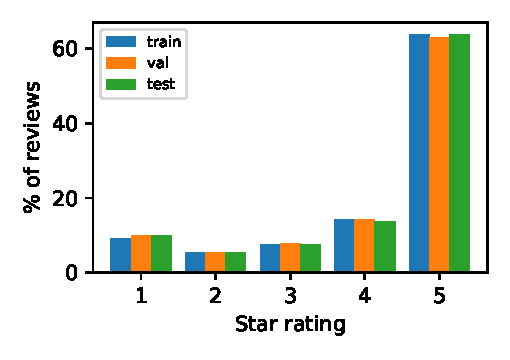
\includegraphics[width=\columnwidth]{rating_distribution.pdf}
\caption{Rating distribution in each split.}
\label{fig:rating}
\end{figure}

\begin{figure}[t]
\centering
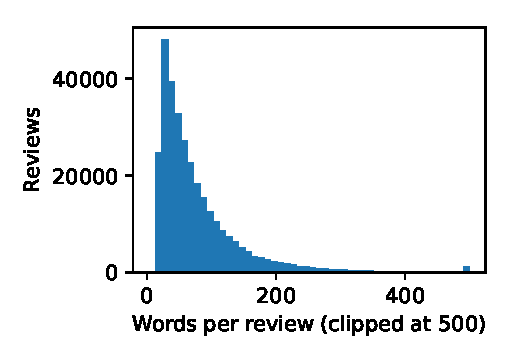
\includegraphics[width=\columnwidth]{review_length.pdf}
\caption{Review length in words (training set, clipped at 500).}
\label{fig:length}
\end{figure}

\subsection{Pilot Experiments}
Before the main runs we measured training time and memory on subsets. TextCNN is cheap: one epoch over the full training set takes about 45--70 seconds and the peak GPU memory is 0.23\,GB. DistilBERT is much more expensive. Fine-tuning on 20{,}000 reviews for one epoch took 155 seconds with every review padded to 256 word pieces, and 102 seconds with dynamic padding (a reduction of about one third), at a peak GPU memory of 2.7\,GB. Extrapolated from this pilot, one epoch over the full training set would take about 27 minutes. We therefore chose to train DistilBERT on a 100{,}000-review subset for two epochs in this report. In practice, an epoch on this subset took 20 to 30 minutes, much longer than the roughly 9 minutes the extrapolation suggested. Part of the gap is the evaluation on the full validation set after every epoch; we did not look into the rest. With the measured speed, a full epoch would take an hour or more, and three losses with three seeds and two epochs on the full training set would take more than 20 hours, so the subsample is needed to finish in the time we have.

\subsection{Main Results}
Table~\ref{tab:main} lists the test results of all six settings. The test set was used once per run, with the checkpoint that had the best validation Macro F1.

\begin{table*}[t]
\caption{Test results (seed 0; mean $\pm$ std once several seeds are available). Lower is better for MAE and large error rate; higher is better for accuracy and Macro F1. Train time is in minutes.}
\label{tab:main}
\centering
\begin{tabular}{llcccccc}
\toprule
Model & Loss & Seeds & Accuracy & Macro F1 & MAE & Large Err. & Train (min) \\
\midrule
\multirow{3}{*}{TextCNN} & CE & 1 & 0.747 & 0.495 & 0.395 & 0.085 & 5.4 \\
 & OLL & 1 & 0.733 & 0.508 & 0.373 & 0.070 & 7.0 \\
 & MLL & 1 & 0.744 & 0.509 & 0.378 & 0.076 & 8.2 \\
\midrule
\multirow{3}{*}{DistilBERT} & CE & 1 & 0.767 & 0.575 & 0.311 & 0.051 & 51.7 \\
 & OLL & 1 & 0.746 & 0.556 & 0.320 & 0.048 & 43.3 \\
 & MLL & 1 & 0.760 & 0.574 & 0.317 & 0.052 & 39.3 \\
\bottomrule
\end{tabular}

\end{table*}

\paragraph{TextCNN.} Both ordinal losses reduce the distance-based errors compared with cross entropy. OLL lowers the MAE from 0.395 to 0.373 and the large error rate from 8.5\% to 7.0\%, and MLL gives 0.378 and 7.6\%. Macro F1 does not drop; it rises slightly from 0.495 to 0.508 (OLL) and 0.509 (MLL). The price is a lower accuracy for OLL (74.7\% to 73.3\%), while MLL stays close to cross entropy (74.4\%). OLL and MLL also trained somewhat more slowly than cross entropy in our runs (Table~\ref{tab:main}); we have not checked whether this comes from the loss itself or just from how busy the GPU was.

\paragraph{DistilBERT.} Here the ordinal losses do not help on the main distance metric. Cross entropy gives MAE 0.311 and a large error rate of 5.1\%. OLL raises the MAE to 0.320 (+2.8\%) and lowers the large error rate only to 4.8\% ($-6.7\%$), while Macro F1 falls from 0.575 to 0.556 and accuracy from 76.7\% to 74.6\%. MLL is close to cross entropy on all metrics (MAE 0.317, large error rate 5.2\%, Macro F1 0.574, accuracy 76.0\%). The OLL run reached its best validation Macro F1 after the first epoch, whereas the other two runs did so after the second. The differences between the three losses are small, and with only one seed we cannot tell which of them are real. Train times in Table~\ref{tab:main} should not be compared between losses, because the GPU was shared with other work to different degrees during the runs.

\paragraph{Architectures.} DistilBERT is clearly stronger than TextCNN with every loss, even though it saw only 100{,}000 training reviews for two epochs, against 314{,}504 reviews for six epochs for TextCNN. With cross entropy its Macro F1 is 0.575 against 0.495, its MAE 0.311 against 0.395, and its large error rate 5.1\% against 8.5\%. The benefit of an ordinal loss is also smaller for the stronger model: the large error rate of TextCNN falls by 17.4\% with OLL, whereas that of DistilBERT falls by 6.7\%, and the MAE does not improve at all. One possible reason is that DistilBERT already makes few large errors with cross entropy, so there is less to gain, but our data cannot confirm this.

\subsection{Reference Baselines}
\label{sec:baselines}
To put the neural results in context, we also trained three simple non-neural references on the same splits: a majority predictor (always 5 stars) and a linear classifier on TF-IDF features of word unigrams and bigrams (at most 60{,}000 features, minimum document frequency 3, sublinear term frequency), trained with stochastic gradient descent on a logistic loss. The linear classifier was fitted once without class weights and once with class weights inversely proportional to the training class frequencies. The settings were fixed in advance and not tuned; three seeds were run, and their standard deviations are about 0.001 or less on all metrics. Table~\ref{tab:baselines} lists the test results.

\begin{table}[t]
\caption{Test results of the non-neural reference baselines (TF-IDF: mean of three seeds).}
\label{tab:baselines}
\centering
\begin{tabular}{lcccc}
\toprule
Baseline & Accuracy & Macro F1 & MAE & Large Err. \\
\midrule
Majority (always 5 stars) & 0.636 & 0.156 & 0.839 & 0.226 \\
TF-IDF, unweighted & 0.733 & 0.450 & 0.456 & 0.104 \\
TF-IDF, class-balanced & 0.729 & 0.528 & 0.408 & 0.081 \\
\bottomrule
\end{tabular}

\end{table}

Two things matter for reading the main results. First, the majority predictor reaches 63.6\% accuracy but a Macro F1 of only 0.156, which confirms that accuracy alone is misleading on this data. Second, class weights alone change the distance-based errors quite a bit: compared with the unweighted linear model, the weighted one lowers the MAE from 0.456 to 0.408 ($-10.4\%$) and the large error rate from 10.4\% to 8.1\% ($-22\%$), and raises Macro F1 from 0.450 to 0.528, with no ordinal information at all. These gains are at least as large as those of OLL and MLL over unweighted cross entropy for TextCNN (Table~\ref{tab:main}). The linear model with class weights is also close to TextCNN with cross entropy (MAE 0.408 against 0.395, large error rate 8.1\% against 8.5\%) and has a higher Macro F1 (0.528 against 0.495). Part of the benefit of the ordinal losses for TextCNN may therefore come from reducing the bias towards the majority class and not from their use of the rating order. We have not yet run cross entropy with class weights on the neural models, which is the control we need to separate the two effects, so it is on our list of remaining work. DistilBERT is clearly better than all three baselines.

\subsection{Error Analysis}
\label{sec:errors}
Figure~\ref{fig:confusion_textcnn} shows row-normalized confusion matrices of the TextCNN models. With cross entropy, the model strongly favors the majority class: 76\% of all test reviews are predicted as 5 stars, although only about 64\% are 5-star reviews. It sends 72\% of the true 4-star reviews, 34\% of the 3-star reviews and 13\% of the 1-star reviews to 5 stars. At the other end, 41\% of the true 2-star reviews are predicted as 1 star, and only 20\% are recognized correctly.

OLL changes this pattern the way it is supposed to. It predicts 5 stars less often (71\% of all reviews), and the large confusions drop: 1-star reviews predicted as 5 stars fall from 13\% to 7\%, and 3-star reviews predicted as 5 stars from 34\% to 20\%. The mistakes move to neighboring ratings instead; for example, the recall of the 2-star class rises from 20\% to 39\% and that of the 4-star class from 14\% to 23\%. This comes at a cost for the extreme classes, whose recall falls (1 star: 77\% to 62\%; 5 stars: 97\% to 93\%), which explains the lower accuracy of OLL. MLL lies between the two, with a pattern closer to cross entropy for the 4-star and 5-star classes.

Figure~\ref{fig:error_distance_textcnn} shows the same trend as the share of test reviews that are off by 0 to 4 stars. Compared with cross entropy, OLL has more errors of exactly one star (19.7\% vs.\ 16.8\%) but fewer errors of three stars (1.4\% vs.\ 1.6\%) and four stars (1.1\% vs.\ 2.1\%). This is the trade-off an ordinal loss is meant to make: it accepts more small errors to get fewer large ones.

\begin{figure*}[t]
\centering
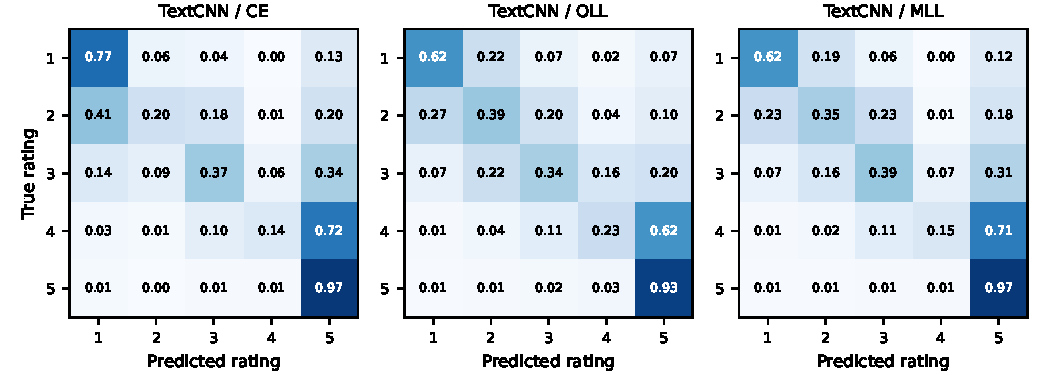
\includegraphics[width=\textwidth]{confusion_textcnn.pdf}
\caption{Row-normalized confusion matrices of the TextCNN models on the test set (rows: true rating, columns: predicted rating).}
\label{fig:confusion_textcnn}
\end{figure*}

\begin{figure}[t]
\centering
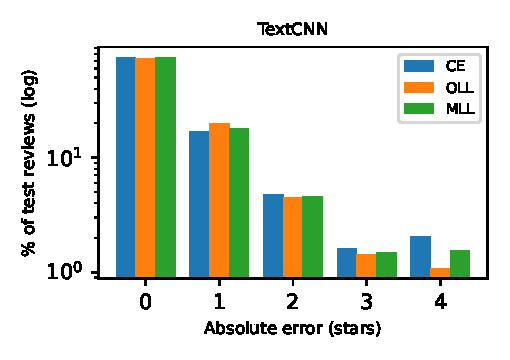
\includegraphics[width=\columnwidth]{error_distance_textcnn.pdf}
\caption{Share of test reviews by absolute error (in stars) for the TextCNN models; the vertical axis is logarithmic.}
\label{fig:error_distance_textcnn}
\end{figure}

\paragraph{Examples.} Table~\ref{tab:examples} shows test reviews on which the TextCNN models behave differently. Among the reviews we inspected in which cross entropy is wrong by three or more stars, several mix positive and negative statements and are pushed into the majority class; the first four rows are of this kind, and OLL (and, in some cases, MLL) predicts a closer rating. Among all 39{,}460 test reviews, 361 are predicted by cross entropy with an error of at least three stars but by OLL within one star, whereas the reverse (OLL off by at least three stars while cross entropy is within one star) happens for 158 reviews. The last two rows are examples of the second case, where OLL fails on reviews that are positive overall. So the gain of OLL on large errors is a net effect, not an improvement everywhere.

\begin{table*}[t]
\caption{Test reviews with different TextCNN predictions (T: true rating; CE, OLL, MLL: predicted rating). Review texts are shown in full.}
\label{tab:examples}
\centering
\small
\begin{tabular}{p{11.5cm}cccc}
\toprule
Review & T & CE & OLL & MLL \\
\midrule
Love the flavor of this gum but the flavor just doesn't last and the gum gets tough quickly. & 2 & 5 & 3 & 5 \\
Seemed like a great idea at first, but these hearts where mushy (overcooked) not good in salads, best in caserole or cooked dished. & 2 & 5 & 3 & 3 \\
They taste good but they'll send you to the toilet quickly and burn you up. There's better beef jerky out there. & 3 & 5 & 4 & 3 \\
The gum is tart and sweet for the initial chew but the flavor is almost gone in ten minutes. & 3 & 5 & 3 & 5 \\
\midrule
We were recommended to use this formula due to severe food allergies to my 5 month old son. His spit-ups stopped after using this and stools also became better. & 5 & 5 & 2 & 5 \\
Hello, The slim jims came in a timely manner, as soon as I expected. Most of them were good, however, I found one of them that was uneatable. & 4 & 3 & 1 & 2 \\
\bottomrule
\end{tabular}
\end{table*}

\paragraph{DistilBERT.} Figures~\ref{fig:confusion_distilbert} and~\ref{fig:error_distance_distilbert} show the same analysis for DistilBERT. The cross-entropy model predicts 5 stars for 67.5\% of the test reviews (64\% are 5-star), much less than TextCNN (76\%). OLL reduces this share to 64.3\% and raises the recall of the 4-star class from 29\% to 42\%, but lowers the recall of 1-star (79\% to 68\%), 2-star (35\% to 29\%) and 3-star (53\% to 47\%) reviews. It has the most one-star errors (20.6\% against 18.2\%) and the fewest errors of four stars (0.4\% against 1.0\%). MLL again lies close to cross entropy.

\begin{figure*}[t]
\centering
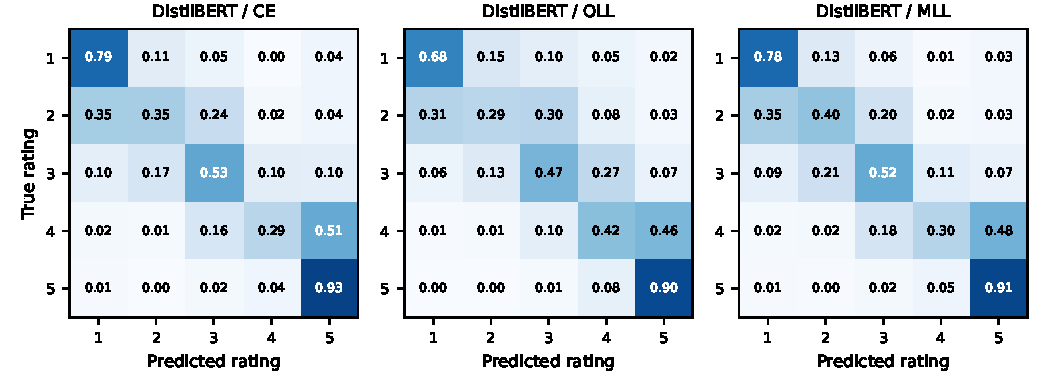
\includegraphics[width=\textwidth]{confusion_distilbert.pdf}
\caption{Row-normalized confusion matrices of the DistilBERT models on the test set.}
\label{fig:confusion_distilbert}
\end{figure*}

\begin{figure}[t]
\centering
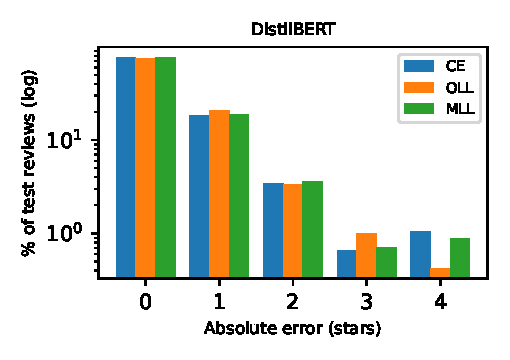
\includegraphics[width=\columnwidth]{error_distance_distilbert.pdf}
\caption{Share of test reviews by absolute error (in stars) for the DistilBERT models; the vertical axis is logarithmic.}
\label{fig:error_distance_distilbert}
\end{figure}

\subsection{Success Criteria Check}
We now check the three conditions from Section~\ref{sec:criteria} against cross entropy. For TextCNN, OLL reduces MAE by 5.4\% and the large error rate by 17.4\% while Macro F1 changes by $+0.013$; MLL reduces MAE by 4.4\% and the large error rate by 10.3\% with a Macro F1 change of $+0.014$. Both therefore meet all three conditions for TextCNN, but only relative to unweighted cross entropy: Section~\ref{sec:baselines} shows that class weights alone can give gains of similar size, so the result may partly reflect the correction of the majority-class bias. This is a single-seed result, so we cannot say yet how much of the difference is just random variation. For DistilBERT, OLL increases the MAE by 2.8\%, reduces the large error rate by 6.7\% and lowers Macro F1 by 0.018, so it meets only the large-error condition and fails the other two. MLL increases the MAE by 1.9\% and the large error rate by 2.3\%, with a Macro F1 change of $-0.0006$; it meets only the Macro F1 condition. The hypothesis is therefore supported for TextCNN but not for DistilBERT in this first run. We will repeat the check with three-seed averages.

\subsection{Cross-Category Evaluation (Optional)}
Not carried out so far; see Section~\ref{sec:conclusion}.

\section{Conclusion and Next Steps}
\label{sec:conclusion}

\subsection{Summary of Work Done}
We built a complete experimental pipeline for predicting 1--5 star ratings from review text. On the Amazon Fine Food Reviews data we removed duplicate reviews (leaving 393{,}135 of 568{,}454) and split the data by product into training, validation and test sets of 314{,}504, 39{,}171 and 39{,}460 reviews, with no product shared between splits. We implemented two architectures, a TextCNN with fixed GloVe embeddings and a fine-tuned DistilBERT, and three loss functions: cross entropy, Ordinal Log Loss (OLL) and Multitask Log Loss (MLL). We implemented the four evaluation metrics (accuracy, Macro F1, MAE and the large error rate) and a training procedure that selects the checkpoint on the validation set and evaluates the test set once. The MLL definition was checked against the original paper. Each of the six settings (two architectures times three losses) has been run once, and the predictions and checkpoints of every run are stored, so we can do a detailed error analysis.

\subsection{Results Obtained So Far}
With TextCNN, both ordinal losses reduce the distance-based errors compared with cross entropy: OLL lowers the MAE by 5.4\% and the large error rate by 17.4\%, MLL by 4.4\% and 10.3\%, and Macro F1 does not drop (it rises by about 0.013). This meets the three success conditions of the proposal for TextCNN, relative to unweighted cross entropy. A class-weighted linear baseline obtains gains of similar size without any ordinal loss (Section~\ref{sec:baselines}), so part of the benefit may come from reducing the bias towards 5 stars. The confusion matrices show why: cross entropy sends most 4-star reviews and many 1- and 3-star reviews to the majority class of 5 stars, whereas OLL spreads its errors to neighboring ratings and makes fewer errors of three or four stars, at the cost of a lower recall for the extreme classes and a lower accuracy (OLL) or an almost unchanged one (MLL).
With DistilBERT (100k training reviews, two epochs) all metrics are better than with TextCNN, but the ordinal losses do not help: OLL raises the MAE from 0.311 to 0.320 and lowers Macro F1 from 0.575 to 0.556, with a small drop in the large error rate (5.1\% to 4.8\%), and MLL is about equal to cross entropy. The hypothesis that ordinal losses reduce distance-based errors is thus supported for TextCNN but not, in this first run, for DistilBERT, so the benefit seems to depend on the architecture and on how strong the baseline already is.
All results come from a single random seed, so they are preliminary.

\subsection{Limitations of the Current Results}
(i)~Every setting has been run once, so we cannot yet quantify random variation, and small differences (for example in the large error rate of DistilBERT) may not be meaningful. (ii)~DistilBERT was trained on a 100{,}000-review subsample for two epochs, because of the time cost on our hardware, whereas TextCNN used the full training set; the architectures are therefore compared under different data budgets. (iii)~The loss parameters $\alpha=1$ and $\lambda=0.5$ and the learning rates were fixed and not tuned on the validation set. (iv)~TextCNN reached its best validation score in the last of its six epochs, so it may be undertrained.

\subsection{Remaining Work}
\begin{itemize}
\item Run each of the six settings with three random seeds and report means and standard deviations, then repeat the success-criteria check on the averages.
\item Tune the main hyperparameters on the validation set with a comparable budget for each loss: $\lambda$ for MLL, $\alpha$ for OLL, and the number of epochs.
\item Train DistilBERT on more (or all) training reviews if time allows, to remove the data-budget difference to TextCNN.
\item Run cross entropy with class weights on both architectures as an additional control, to separate the effect of the ordinal losses from that of correcting the class imbalance.
\item Extend the error analysis with examples of misclassified reviews, especially reviews with mixed opinions, and compare the training times of the losses.
\item Optionally, evaluate the trained models on reviews from another product category to examine generalization~\cite{blitzer2007}.
\item Prepare the final report.
\end{itemize}


\bibliographystyle{IEEEtran}
\bibliography{references}

\end{document}
